\subsection{Poisson}
Nochmal: die grundlegende Annahme von Seung-Hoon Na und Hwee Tou Ng lautet:\\
\fbox{ 
\begin{minipage}{12cm}
	``Our key assumption is that the frequency of anaphoric expressions is distributed over named entities in a document according to the probabilities of whether the document is elite for the named entities.''\cite{paper:Na}
\end{minipage}
}\\
\\
Um diese Annahme in ein mathematisches Modell zu übersetzen, muss man die Wahrscheinlichkeit abschätzen, dass ein Dokument ``elite'' ist. Wir suchen also eine Formel für
\[P\left( E\left( e \right)=1|d \right)=\ ?\]
Zunächst interessiert uns hierfür die Wahrscheinlichkeit, dass eine beliebige Entität $tf$-fach in einem Dokument vorkommt. Dafür wird ein 2-Poisson Mixture Modell herangezogen.

\begin{equation}
P\left( tf \right)=\pi_e\frac{e^{-\lambda_e}\lambda_{e}^{ tf }}{tf!}+\left( 1-\pi_e \right)\frac{e^{-\mu_e} \mu_e^{tf}}{tf!}
\end{equation}
Der erste Term repräsentiert hierbei die Wahrscheinlichkeit des $tf$-fachen Auftretens der Entität in der Funktion als ``elite''-Eigennamen, der zweite Term steht für die Wahrscheinlichkeit des tf-fachen Auftretens der Entität als ``non-elite''-Eigennamen.
\[P\left( tf \right)=\underbrace{\pi_e\frac{e^{-\lambda_e}\lambda_{e}^{ tf }}{tf!}}_{Wahrscheinlichkeitsanteil - elite} +\underbrace{\left( 1-\pi_e \right)\frac{e^{-\mu_e} \mu_e^{tf}}{tf!}}_{Wahrscheinlichkeitsanteil - nonelite}\]
Dabei deutet $\pi_e$ auf den Erwartungswert hin, ob ein Dokument ``elite'' ist oder nicht.\\
$\pi_e$, $\lambda_e$ und $\mu_e$ werden festgelegt als:
\[\pi_e=\frac{df\left( e \right)}{df\left( e \right)+N}, \ \lambda_e=\frac{cf\left( e \right)}{df\left( e \right)}, \ \mu_e=\frac{cf(e)}{N}\]
wobei
\begin{itemize}
	
	\item $N$: Anzahl der Dokumente
	\item $df(e)$: Anzahl der Dokumente, in denen $e$ vorkommt
	\item $cf(e)$: Anzahl von $e$ in allen Dokumenten
\end{itemize}
Damit haben wir ein Modell, dass die Wahrscheinlichkeit der Häufigkeit von Entitäten in Dokumenten schätzt. Wichtig ist hierbei, dass sowohl das Auftreten von ``elite''-Entitäten in Dokumenten mit einer Poissonverteilung modelliert wird, als auch das ``zufällige'' Auftreten der ``nonelite''-Entitäten.\\
Eine einfache Poissonverteilung sieht in Formel und im Diagramm wie folgt aus:
\[P_\lambda(k)=\frac{\lambda^k}{k!}e^{-\lambda}\]
\begin{table}[h]
	\centering
	\begin{tabular}{c}
		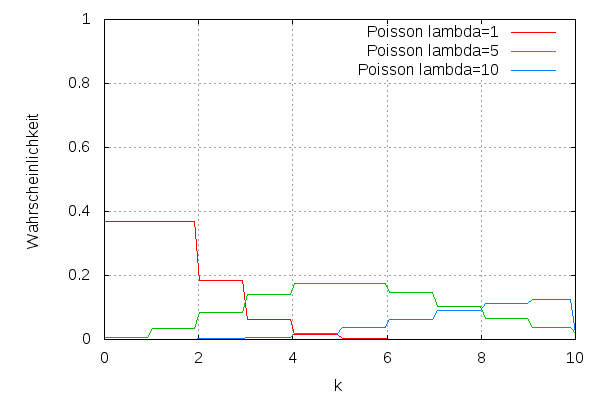
\includegraphics[scale=0.5]{pics/poisson_basic}
	\end{tabular}
	\caption{Einfache Poissonverteilung}
	\label{tab:poisson_basic}
\end{table}

Mit Hilfe von $(1)$ können wir nun $P(\textbf{E}(e)=1|d)$ bestimmen. Wir setzen
\[ P(\textbf{E}(e)=1|d) = \frac{\pi_e P(tf(e;d)|\textbf{E}(e)=1)}{\pi_e P(tf(e;d)|\textbf{E}(e)=1) + (1-\pi_e) P(tf(e;d)|\textbf{E}(e)=0)} \]
mit
\begin{eqnarray*}
	P(tf(e;d)|\textbf{E}(e)=1) &=& \frac{e^{-\lambda_e}\lambda_e^{tf}}{tf!}\\
	P(tf(e;d)|\textbf{E}(e)=0) &=& \frac{e^{-\mu_e}\mu_e^{tf}}{tf!}
\end{eqnarray*}

und erhalten so

\begin{eqnarray*}
	P(\textbf{E}(e)=1|d) 	&=& 	\frac{\pi_e P(tf(e;d)|\textbf{E}(e)=1)}{\pi_e P(tf(e;d)|\textbf{E}(e)=1) + (1-\pi_e) P(tf(e;d)|\textbf{E}(e)=0)} \\
	&=&	\frac{\pi_e \frac{e^{-\lambda_e}\lambda_e^{tf}}{tf!}}{\pi_e \frac{e^{-\lambda_e}\lambda_e^{tf}}{tf!} + (1 - \pi_e) \frac{e^{-\mu_e}\mu_e^{tf}}{tf!}}\\
	&=&	\frac{\pi_e{e^{-\lambda_e}\lambda_e^{tf}}}{\pi_e {e^{-\lambda_e}\lambda_e^{tf}} + (1 - \pi_e) e^{-\mu_e}\mu_e^{tf}}\\
	&=&	\frac{\pi_e}{\pi_e + (1-\pi_e)\frac{e^{-\mu_e}\mu_e^{tf}}{e^{-\lambda_e}\lambda_e^{tf}}}\\
	&=&	\frac{\pi_e}{\pi_e + (1-\pi_e)e^{\lambda_e - \mu_e}\left( \frac{\mu_e}{\lambda_e}\right)^{tf(e;d)}}	
\end{eqnarray*}

Jetzt werden 2 Fälle unterschieden:
\begin{enumerate}
	\item $e=e_Q$ \\
		Wir machen die plausible Annahme, dass $tf(e;d) \geq 1$, wenn das Dokument $d$ elite ist für die gesuchte Entität $e$. Alle anderen Dokumente im Test seien non-elite bezüglich $e$. \\
		Dann können wir die $\pi_e, \lambda_e \text{ und } \mu_e$ wie oben beschrieben ersetzen und erhalten
		\begin{eqnarray*}
			P(\textbf{E}(e)=1|d)	&=&	\frac{\pi_e}{\pi_e + (1-\pi_e)e^{\lambda_e - \mu_e}\left( \frac{\mu_e}{\lambda_e}\right)^{tf(e;d)}}\\
			&=&	\frac{\frac{df(e)}{df(e) + N}}{\frac{df(e)}{df(e) + N} + \left(1-\frac{df(e)}{df(e) + N}\right) e^{\frac{cf(e)}{df(e)}-\frac{cf(e)}{N}} \left( \frac{\frac{cf(e)}{N}}{\frac{cf(e)}{df(e)}}\right)^{tf(e;d)}}\\
%			&=&	\frac{1}{1 + \frac{e^{\frac{cf(e)}{df(e)}-\frac{cf(e)}{N}}\left( \frac{df(e)}{N}\right)^{tf(e;d)}}{\frac{df(e)}{df(e) + N}} - e^{\frac{cf(e)}{df(e)}-\frac{cf(e)}{N}}\left( \frac{df(e)}{N}\right)^{tf(e;d)} }\\
			&=&	\frac{1}{1+ \left( \frac{df(e)}{N}\right)^{tf(e;d)-1}e^{\frac{cf(e)}{df(e)}-\frac{cf(e)}{N}}}
		\end{eqnarray*}
\end{enumerate}
